In this chapter we present our impressions on the User Experience of the tested project. These are opinions from a user point of view that we hed during test and usage of the system.

\subsection{Login Page}

In our opinion the login page, strongly empowered by the large usage of JavaScript, is good looking even if it does not follow the colour scheme and the general look of the calendar page found once logged into the system. \\
We found some problems in case of invalid signup: if you insert some invalid data, such as a password too short or too similar to the username, the system redirects you to the login form instead of the signup one, which is slightly annoying.

\begin{center}
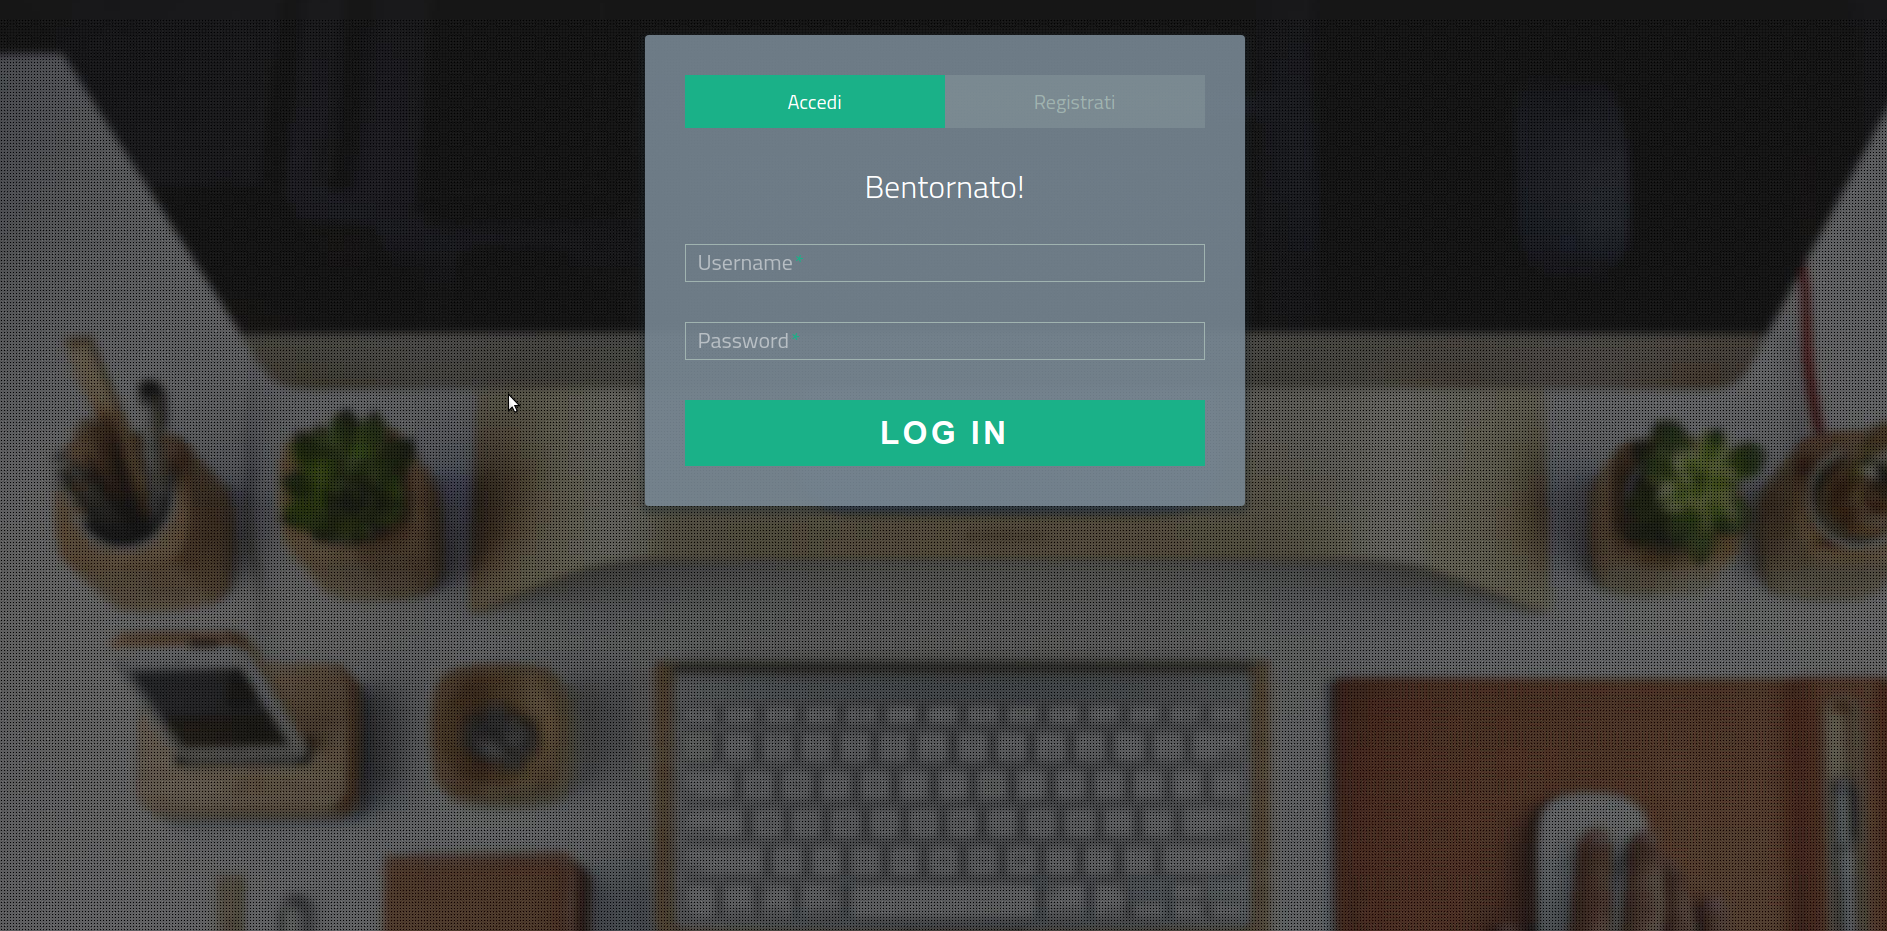
\includegraphics[width=\textwidth]{Images/LoginPage}
\end{center}

\subsection{Calendar Main Page}

The calendar page of the system that goes through daily, weekly and monthly views of the calendar, in spite of being similar to Google Calendar page, is really immediate and provides everything you need. \\
For what concerns the form that allows a user to create a appointment, we found that the procedure used to insert dates and the location is not very user-friendly: locations are not suggested, for example using Google API, although these API are used later to retrieve longitude and latitude from the name of location inserted; to insert a starting and ending date for an event, you have to provide always a full date format (e.g. '2018-01-10 10:30') and after a few uses it becomes very uncomfortable, especially being used to select dates from datepickers.

\begin{center}
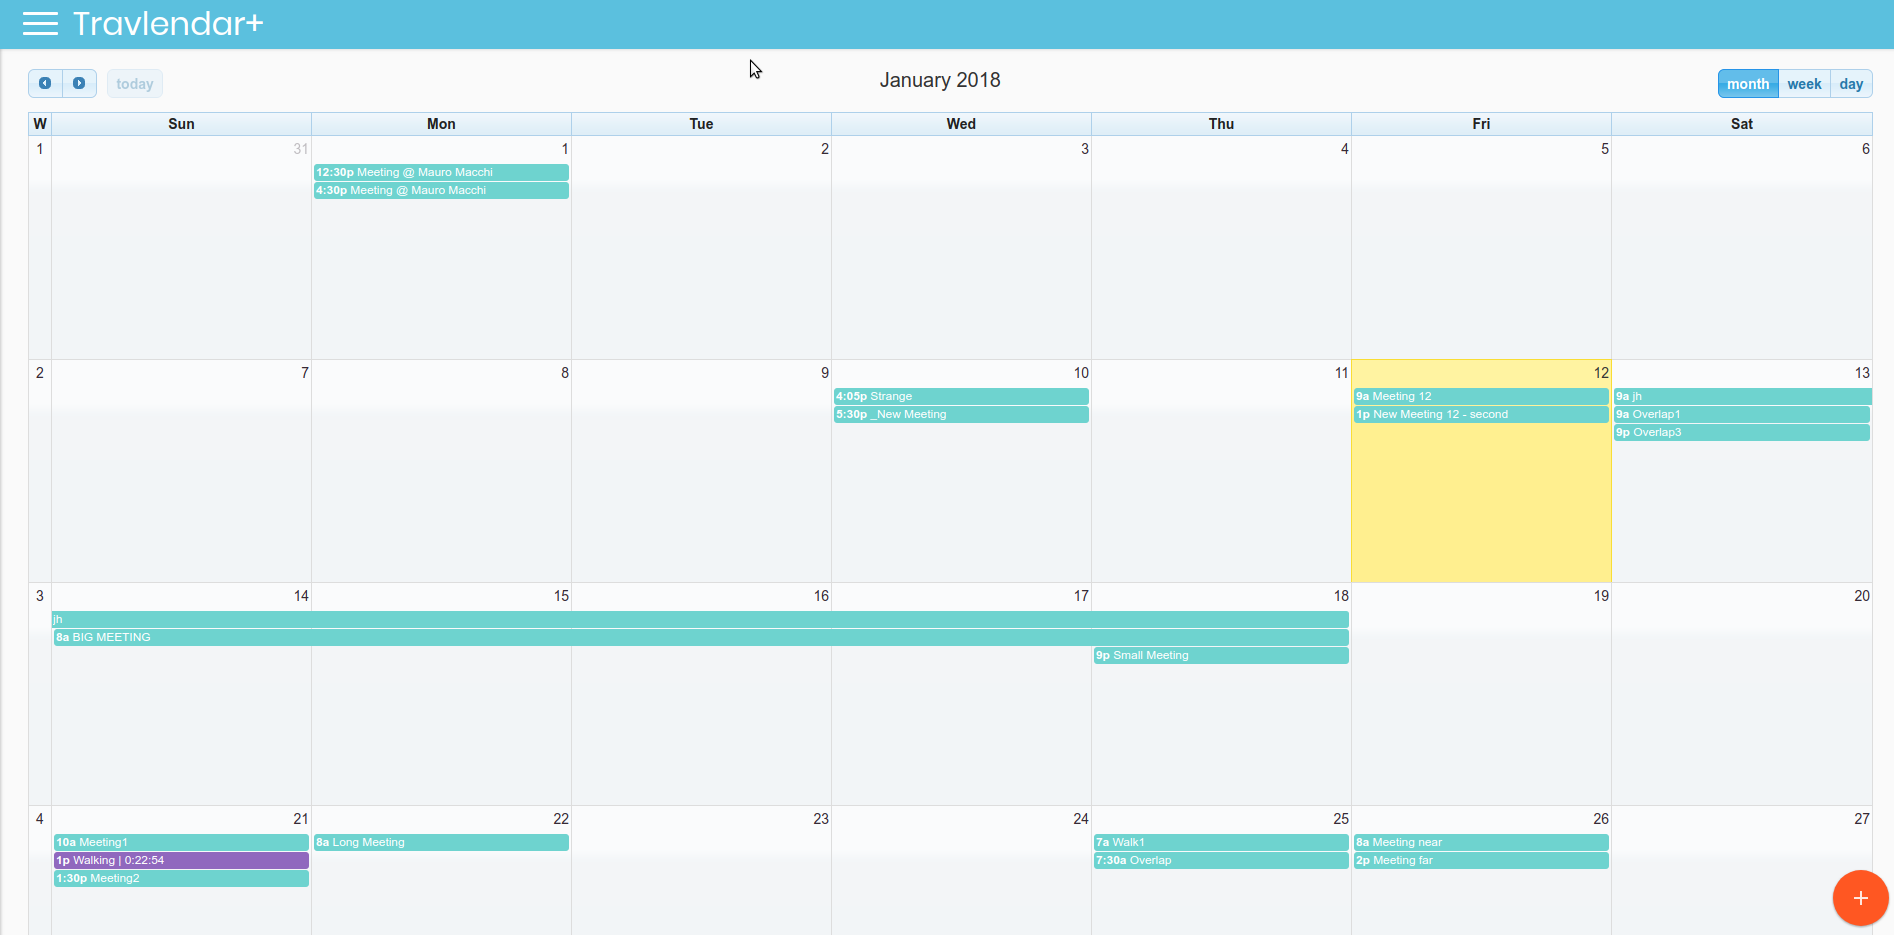
\includegraphics[width=\textwidth]{Images/CalendarPage}
\end{center}

\subsection{General Considerations}
\begin{itemize}
	\item Breaks are fixed from 12.00 to 14.00 and when one or more appointments overlap with them and make them not doable, it is signalled using a window alert. This procedure is done correctly by the system. However, in spite this is written in a requirement on the RASD document of the project, we believe that not to give the possibility to create customizable breaks is limiting for a complete and satisfying usage of Travlendar+. In addition, the system signalled you that a break is not doable only when it actually becomes not doable and you can not check it anymore afterwards. It is also not possible to see the computed starting times for breaks that are actually doable.
	\item When two appointments overlap, the system signals it with a warning using a window alert and deletes the appointment that has just create the warning. In our opinion not letting you to create this event is a strong choice, e.g. the second appointment is much more important so you want to sacrifice the former, or you want to take them both. Travlendar should have taken it into account and at least give you the possibility to choose which one to delete or create a separate page where all these warnings, maybe together with not doable breaks, are listed.
	\item~While testing the application we have also found a little bug: if you try to create two different appointments in two locations whose names are not the same, but that get geocoded to the same latitude-longitude pair (for example "Duomo Milano" and "Duomo di Milano"), than the second appointment is not correctly created and the application's execution flow stops. This is probably because of a unique constraint failing at the database level.
\end{itemize}